\documentclass[12pt]{article}

\usepackage{sbc-template}
\usepackage{graphicx,url}
\usepackage[utf8]{inputenc}

\usepackage{verbatim}
\usepackage{xspace}
\newcommand{\FC}       {Freechains\xspace}
\newcommand{\reps}     {\emph{reps}\xspace}
\newcommand{\onerep}   {\emph{1~rep}\xspace}
\newcommand{\nreps}[1] {\emph{#1~reps\xspace}}
\newcommand{\code}[1]  {\texttt{\footnotesize{#1}}}
\newcommand{\Xon} {$1{\rightarrow}N$\xspace}
\newcommand{\Xno} {$1{\leftarrow}N$\xspace}
\newcommand{\Xnn} {$N{\leftrightarrow}N$\xspace}
\newcommand{\Xoo} {$1{\leftrightarrow}1$\xspace}
\newcommand{\Xo}  {$1{\hookleftarrow}$\xspace}

\renewcommand{\theenumi}{\alph{enumi}}

\hyphenation{off-line}

\sloppy

\title{
    Peer-to-Peer Permissionless Consensus via Reputation
}

\author {
    Francisco Sant'Anna,
    Fabio Bosisio,
    Lucas Pires
}
\address {
    UERJ - PEL - Pós-Graduação em Engenharia Eletrônica
    \email{francisco@ime.uerj.br, fbosisio@gmail.com, lucasampires@gmail.com}
}

\begin{document}

\maketitle

\begin{abstract}
Public Internet forums suffer from excess and abuse, such as SPAM and fake
news.
Centralized platforms employ filtering and anti-abuse policies, but imply full
trust from users.
%
We propose a permissionless Sybil-resistant peer-to-peer protocol for content
sharing.
Our main contribution is a reputation system that moderates content and, at the
same time, delivers network consensus.
We can trace a parallel with Bitcoin as follows:
    consolidated posts create reputation (vs proof-of-work),
    likes and dislikes transfer reputation (vs transactions), and
    aggregate reputation determines consensus (vs longest chain).
%
The reputation mechanism depends exclusively on the human authoring ability
(\emph{proof-of-authoring}), which is slow and scarce, thus suitable to
establish consensus.
\end{abstract}

\begin{comment}
\begin{resumo} 
Fórums públicos de Internet sofrem de excesso e abuso, tais como SPAM e
notícias falsas.
Plataformas centralizadas adotam políticas de filtragem e anti abuso, mas
exigem confiança dos seus usuários.
%
Nós propomos um protocolo peer-to-peer não permissionado para compartilhamento
de conteúdo que é resistente a ataques Sybil.
Nossa principal contribuição é um sistema de reputação que serve para moderar o
conteúdo e ao mesmo tempo garantir consenso na rede.
%
Nós traçamos um paralelo com o Bitcoin da seguinte forma:
    postagens consolidadas criam reputação (vs \emph{proof-of-work}),
    \emph{likes} e \emph{dislikes} transferem reputação (vs transações), e
    a reputação agregada determina o consenso (vs cadeia mais longa).
%
O mecanismo de reputação depende exclusivamente da habilidade de autoria humana
(\emph{proof-of-authoring}), que é lenta e escassa, e portanto adqueada para
estabelecer consenso.
\end{resumo}
\end{comment}

\section{Introduction}
\label{sec.introduction}

Content publishing in Internet forums and social media is
increasingly more centralized in a few companies (e.g. Facebook and
Twitter)~\cite{internet.fixing}.
%,p2p.osn,p2p.dosn}.
%These companies benefit from closed protocols and network effects to keep
%users locked in their platforms.
These companies offer free storage, friendly user interfaces, and robust access,
but concentrate excessive power, controlling and monetizing over private user data.
%
Peer-to-peer alternatives~\cite{p2p.survey} eliminate intermediaries, but
strive to achieve consistency when dealing with malicious users.
%given the decentralization of authority and infrastructure.
% and push to end users the responsibility to manage data and connectivity.

In an ideal Internet forum, all messages or posts
(i)   reach all users,
(ii)  are delivered in consistent order, and
(iii) are respectful and on topic.
In centralized systems, items (i) and (ii) are trivially achieved assuming
availability and delivery order, while item (iii) requires that users trust the
service to moderate content.
In decentralized systems, however, none of these demands are easily
accomplished.
A common approach in gossiping protocols is to proactively disseminate posts
among peers until they reach all users~\cite{p2p.survey,p2p.byz}.
However, gossiping does not guarantee consensus since posts can be received in
conflicting orders~\cite{p2p.intention}.
%,p2p.dvcs}.
%As an example, antagonistic messages such as \emph{"X is final"} vs
%\emph{"Y is final"} might be sent concurrently, preventing the network to
%determine as a group its intention as \emph{X} or \emph{Y}.
%
Consensus is key to distinguish malicious behavior \emph{at the protocol
level}, and therefore, satisfy item (iii).
Without consensus, each client must rely on local anti-abuse policies, such as
SPAM filters and blacklists, but which only apply a posteriori, when the
abusive messages have already been flooded in the network by potential
Sybils~\cite{p2p.sybil}.
%
%fundamental in collaborative applications, such as open discussion
%forums, chat rooms, and trading services (e.g., delivery \& auction).
%Otherwise, they become impractical due to excess and abuse (e.g., SPAM and
%illicit content).
%At the very core, consensus is

\begin{comment}
Consensus is notably challenging to the point that decentralized protocols
partially abdicate of it.
%For instance, it is typically either possible to have
%\emph{multi-user/single-node} or \emph{single-user/multi-node}, but not
%\emph{multi-user/multi-node} consensus:
%
On the one hand, federated protocols~\cite{p2p.ecosystem} offer
\emph{multi-user/single-node consensus}, in which multiple users can exchange
messages consistently within a single trusted server, but not globally across
multiple servers.
%
On the other hand, a protocol like Scuttlebutt~\cite{p2p.scuttlebutt} offers
\emph{single-user/multi-node consensus}, in which a single user has full
authority over its own content across machines, but multiple users cannot reach
consensus even in a local machine.
%
Our goal is to provide \emph{multi-user/multi-node consensus} (just
\emph{consensus}, from now on) in the context of decentralized content sharing.

In this sense, consensus 
eradicate Sybil, which are the
major threat to decentralized applications in general.
The reason
Furthermore, without consensus, it is not possible,
\end{comment}

Bitcoin~\cite{p2p.bitcoin} is the first permissionless protocol to resist
Sybil attacks, relying on a scarce resource---the \emph{proof-of-work}---to
establish consensus.
%The protocol maintains a single dispendious timeline consisting of linked
%blocks with transactions, which represent the consensus.
%Alternative timelines need to spend more resources to substitute the consensus.
The protocol is Sybil resistant because it is expensive to write to its
unique timeline (either via proof-of-work or transaction fees).
%
However, Bitcoin and cryptocurrencies in general are not suitable for social
content sharing because
    (i)   they enforce a unique timeline to preserve value and immunity to
          attacks;
    (ii)  they lean towards concentration of power due to scaling effects;
    (iii) they impose an external economic cost to use the protocol; and
    (iv)  they rely exclusively on objective rules to reach consensus.
%
These issues threaten our original decentralization goals, and more
importantly, they renounce subjectivity, which is inherent to content
moderation.
%
For instance, a unique timeline implies that all Internet content should be
subject to the same consensus rules, while objective rules alone cannot
distinguish abuse amid content.
%
Another limitation of cryptocurrencies is that it is not possible to revoke
content in the middle of a blockchain, which is inadmissible considering
illicit content (e.g., hate speech)~\cite{btc.content}.
%For instance, Bitcoin transactions permanently store arbitrary human-authored
%content, including harmful texts and images.
%~\cite{btc.data}

In this work, we adapt the idea of scarce resources to reach consensus and
eradicate Sybils, but in the context of social content sharing.
We indicate 4 main contributions:
%
\begin{enumerate}
\item Recognizing published contents as scarce resources, since they require
human work.
Work is manifested as new posts, which if approved by others, reward authors
with reputation tokens, which are further used to evaluate other posts with
likes and dislikes.
With such \emph{proof-of-authoring} mechanism, token generation is expensive,
while verification is cheap and shared by multiple users.
%
\item Using the reputation system to determine consensus.
Due to decentralization and network partitions, posts in a timeline form a
causal graph with only partial order, which we promote to a total order based
on the reputation of authors.
The consensus order is fundamental to detect conflicting operations, such as
likes with insufficient reputation (akin to Bitcoin's double spending).
%
\item Allowing users to create diversified forums of interest (instead of a
singleton blockchain), each counting as an independent timeline with its own
subjective authoring etiquette.
%
\item Supporting content removal without compromising the integrity of the
decentralized blockchain.
Users have the power to revoke posts with dislikes, and peers are forced to
remove payloads, only forwarding associated blockchain metadata.
\end{enumerate}
%
We integrated the proposed consensus algorithm into \FC~\cite{fcs.sbseg20}, a
practical peer-to-peer (P2P) content dissemination protocol that provides
strong eventual consistency~\cite{p2p.sec}.
%p2p.crdts,
To show the feasibility of the consensus mechanism, we simulated months of
activity of a chat channel and years of a newsgroup forum, both extracted from
publicly available Internet archives.

The rest of the paper is organized as follows:
In Section~\ref{sec.design}, we describe the design of the reputation and
consensus mechanism for public forums and discuss some security threats.
In Section~\ref{sec.freechains}, we describe the concrete reputation rules we
implemented for \FC and evaluate the performance of the protocol in real-world
public forums.
In Section~\ref{sec.related}, we compare our system with publish-subscribe
protocols, federated applications, and fully P2P systems.
In Section~\ref{sec.conclusion}, we conclude this work.

\section{The Reputation and Consensus Mechanism}
\label{sec.design}

In the absence of moderation, permissionless P2P forums are impractical, mostly
because of Sybils abusing the system.
For instance, it should take a few seconds to generate thousands of fake
identities and SPAM millions of messages.
%Hence, without moderation, there are no limits on the number and size of posts
%and no reasonable policy to distinguish quality.
For this reason, we propose a reputation system that works together with a
consensus algorithm to resist Sybil attacks.
% and make peer-to-peer public forums practical.
We consider Sybils to be groups of throw-away identities and machines with no
previous reputation in the forums.

In our system, users can spend tokens named \reps to post and rate content in
forums:
a \code{post} initially penalizes authors until it consolidates and counts
positively;
a \code{like} is a positive feedback that helps subscribers to distinguish
content amid excess;
a \code{dislike} is a negative feedback that revokes content when crossing a
threshold.
Table~\ref{fig.general} summarizes the general reputation rules and their
goals.
To prevent Sybils, users with no \reps cannot operate under these rules,
requiring a welcoming like from any other user already in the system.
The fact that likes are zero-sum operations, which only transfer reputation,
eliminates the incentives from malicious users to invite Sybils into the
system.
The only way to generate new \reps is to post content that other users
tolerate, which demands non-trivial work resistant to automation.%
\footnote{
    Note that although human and AI content may become indistinguishable, their
    frequency and relevance in forums is still subject to human evaluation in
    our proposal.
}
In this sense, having one or hundreds of machines in the network does not
affect the capacity to write into the forums.

\begin{table}
\centering
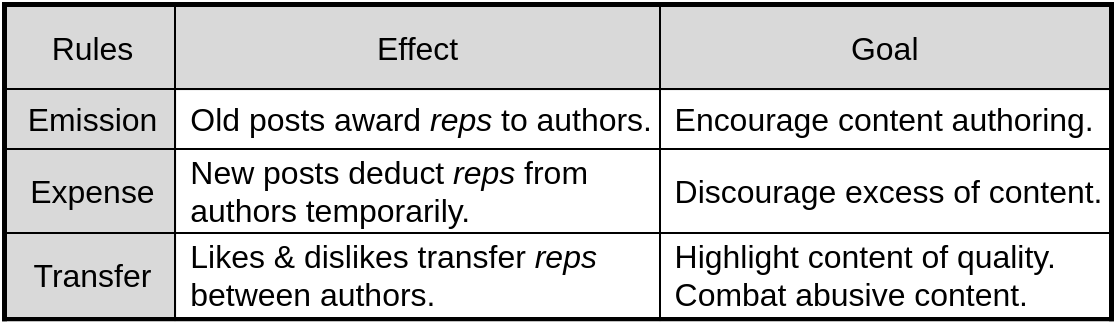
\includegraphics[width=0.65\textwidth]{general.png}
\caption{General reputation rules in public forums.}
\label{fig.general}
\end{table}

Bitcoin employs proof-of-work to mitigate Sybil attacks.
However, CPU or other extrinsic resources are not evenly distributed among
humans, specially in communications using battery-powered devices.
%
Instead, considering the context of public forums, we propose to take advantage
of the human authoring ability as an intrinsic resource.
Creating new content is hard and takes time, but is comparatively easy to
verify and rate.
Therefore, in order to impose scarcity, we determine that only content
authoring generates \reps, while likes and dislikes only transfer \reps between
users.
%but limited by periods of time to prevent excess (e.g., once in a day per user).
%Additionally,
In our analogy with Bitcoin, Sybil attacks would require to add human resources,
instead of CPU power.

Nevertheless, posts scarcity is not yet sufficient to combat Sybils because
consensual order is still required to prevent inconsistent operations.
For instance, consider a malicious author with a single unit of \reps posting
SPAM messages from multiple peers at the same time.
According to the \emph{Expense} rule of Table~\ref{fig.general}, only one of
these messages should be accepted by the network.
However, without consensus, it is not possible to globally determine which
message to accept, since each peer would supposedly accept the first message it
receives.
On the one hand, in order to validate operations consistently, we need the same
message ordering across all peers in the network.
On the other hand, due to network partitions, we can only represent public
forums as DAGs (directed acyclic graphs) with causal relationships between
messages, which provides at most partial order.

\subsection{Basic Reputation Consensus}
\label{sec.design.basic}

Our key idea to stablish consensus in forum DAGs is to favor forks with posts
from users that constitute the majority of the reputation.
These forks have more associated work and are analogous to longest chains in
Bitcoin.
%
In technical terms, we adapt a topological sorting algorithm to favor
reputation when deciding between branches in a forum DAG.

Figure~\ref{fig.reps}.A illustrates the evolution of a forum DAG in the
presence of a network partition:
A common prefix has signed posts from users $a$, $b$, and $c$, when they were
still all connected.
%
We assume that within the prefix, users $a$ and $b$ have contributed with
better content and therefore have more reputation combined than $c$ has alone
(i.e., $8+5>3$).
We will use this fact to order branches in the consensus algorithm.
%
Then, user $c$ disconnects from $a$ and $b$, and evolves with new users $x$ and
$y$ in \code{branch-1}.
In the meantime, $a$ and $b$ participate with new posts in \code{branch-2}.
After some time, the partitions reconnect and new posts from $x$, $b$ and $c$
merge the branches now with a common suffix.

\begin{figure}
\centering
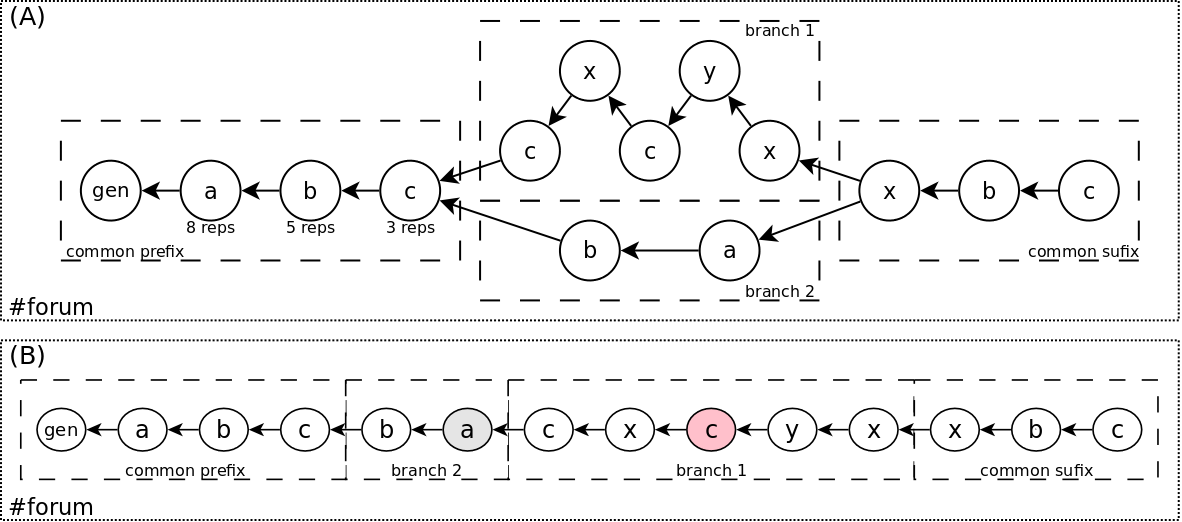
\includegraphics[width=0.9\textwidth]{reps.png}
\caption{
    (A) A public forum DAG with a common prefix, two branches, and a common sufix.
    (B) Total order between posts of the DAG after consensus.
}
\label{fig.reps}
\end{figure}

Note that even non-malicious network partitions may experience conflicts when
merging branches.
For instance, dislike operations in one branch to past posts in the common
prefix could possibly block posts from users in the other branch.
%, depending on how the posts are ordered.
Therefore, we need to order branches with a global consensus, such that we can
validate operations consistently across the network.
%
Note also that, to reach consensus, we should preferably rely on the maximum
information that all branches agree on, which is exactly the posts in the
common prefix.

Based on the reputation of users in the common prefix, Figure~\ref{fig.reps}.B
indicates the consensus order between posts in the forum DAG:
    the common prefix comes first,
    then all posts in \code{branch-2},
    then all posts in \code{branch-1},
    then the common suffix.
%
The \code{branch-2} with users $a$ and $b$ takes priority over \code{branch-1}
with user $c$ because, before the forking point, $a$ and $b$ have more
reputation than $c$, $x$, and $y$ have combined.

The basic consensus rule is therefore straightforward:
Whenever a fork is found, we create sets of users with posts in each branch
($B1=\{c,x,y\}$ and $B2=\{a,b\}$).
Then, we take each set, and sum its users \reps based on the common prefix
($S1=3$ and $S2=13$), since it is the maximum information that all branches
agree.
Finally, we order the branches based on the highest sum of \reps found
(Figure~\ref{fig.reps}.B).

While applying the branches in order, if any post operation fails, all
remaining posts are rejected and removed from the DAG, as if they never
existed.
As an example, suppose that the last post by $a$ in \code{branch-2} (in gray)
is a dislike to user $c$.
Then, it's possible that the last post by $c$ in \code{branch-1} (in red), now
suppose with \nreps{0}, is rejected together with all posts in sequence,
including those in the common suffix.
%
This rejection rule for remaining posts is a direct consequence of tamper proof
Merkle~DAGs~\cite{p2p.ipfs,p2p.bitcoin} typically used in permissionless
protocols, which cannot support graph modifications.

There are some other relevant considerations about forks and merges:
%
Peers that first receive branches with less reputation need to reorder all
posts after the forking point.
This might involve removing content in the end-user software.
This behavior is similar to Bitcoin's blockchain reorganization, when peers
detect new longest chains. % and disconsiders old blocks.
%
Likewise, peers that first saw branches with more reputation just need to
append the other branch, with no reordering at all.
%and do not need to recompute anything.
This behavior is expected to happen in the majority of the connected network.
%
Legitimate posts in secondary branches might be removed due to merges, which
requires that users repost the messages.
Nevertheless, we expect that legitimate users gossip among themselves more
often, preventing this situation.
%
Note that unlike Bitcoin, forks are not only permitted but encouraged due to
the local-first software principle~\cite{p2p.local}, in which networked
applications can work locally while offline.
However, the longer a peer remains disconnected, the more conflicting
operations it may see, and the higher are the chances of posts reordering when
rejoining.

In summary, it is important to remark that
    (i) branches always introduce conflicts, which
    (ii) require consensus to order operations, which
    (iii) is based on a common prefix reputation,
    (iv) leading to a global and deterministic result.
%
Note that the consensus order exists only to account reputation and verify
operations, and is only a view of the primary DAG structure of public forums.

\subsection{Malicious Behaviors and Hard Forks}
\label{sec.design.hard}

Consider a malicious scenario in which user $c$ in Figure~\ref{fig.reps}
intentionally disconnects from the network for weeks to cultivate fake
identities $x$ and $y$ with the intention to accumulate \reps.
When merging, these fake users would become legitimate and take over the
majority of \reps in the forum.
%
However, this kind of attack is refutable because, since the common prefix is
the basis of consensus, users in the branch with more reputation can still
react even a posteriori.
For instance, users $a$ and $b$ can pretend that they did not yet see
\code{branch-1} and post extra dislikes to user $c$ so that a further merge
invalidates all posts from \code{branch-1}, removing them from the DAG.
%
This kind of attack is innocuous because it requires at least half of the \reps
accumulated in the common prefix.
%
%The same countermeasure can be used against a minority of malicious users
%colluding to boost or protect their own posts.

\begin{figure}
\centering
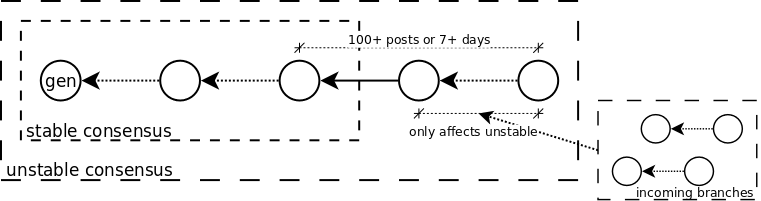
\includegraphics[width=0.85\textwidth]{n100-d7.png}
\caption{
    Stable consensus freezes the order of posts once they cross the threshold.
    The unstable order may still be affected by incoming branches.
}
\label{fig.hard}
\end{figure}

As a counterpoint, maybe users $a$ and $b$ have abandoned the forum for months,
and thus \code{branch-1} is actually legitimate.
In this case, users $a$ and $b$ might be the ones trying to take over the
forum and would succeed, since they control the majority of \reps in the common
prefix.
Yet another possibility is that both branches are legitimate but became
disconnected for a long period of time.
In any case, it is unacceptable that an old remote branch affects a local
active forum.

For this reason, the consensus algorithm includes an extra constraint that
prevents long-lasting local branches to merge, which leads to \emph{hard forks}
in the network.
A hard fork occurs when a local branch crosses a predetermined and irreversible
threshold of \emph{7 days} or \emph{100 posts} of activity.
In this case, regardless of the remote branch reputation, the local branch
takes priority and is ordered first.
This situation is analogous to a hard fork in Bitcoin and the branches become
incompatible and will never synchronize again.
More than simple numeric disputes, a hard fork represents a social conflict in
which reconciling branches is no longer possible.

Figure~\ref{fig.hard} illustrates hard forks by distinguishing \emph{stable
consensus}, which cannot be reordered, from \emph{unstable consensus}, which
may still be affected by incoming branches.
The activity threshold counts backwards, starting from the newest local post
in the unstable consensus to older posts until they are permanently frozen.

In summary, the rules to merge a branch \code{j} from a remote machine into a
branch \code{i} from a local machine are as follows:
\begin{itemize}
    \item \code{i} is first if it crosses the activity threshold of
          \emph{7 days} or \emph{100 posts}, regardless of \code{j}.
    \item \code{i} or \code{j} is first, whichever has more reputation in the
          common prefix, as discussed in Section~\ref{sec.design.basic}.
    \item otherwise, branches use the arbitrary criteria of lexicographical
          order of the post hashes immediately after the common prefix.
\end{itemize}

To conclude this section, we should keep in mind that our consensus algorithm
is based on subjective evaluations of users and posts.
For this reason, unlike Bitcoin, in which forks are discouraged and a single
blockchain must prevail, public forums can split and diverge indiscriminately.
For instance, users can explicitly apply hard forks at any point in time to
``reboot'' a community from a previous state.
Ultimately, the consensus algorithm provides a transparent mechanism to help
users understand the evolution of public forums and act accordingly, even if it
leads to hard forks.

\subsection{Content Removal}

\begin{figure}
\centering
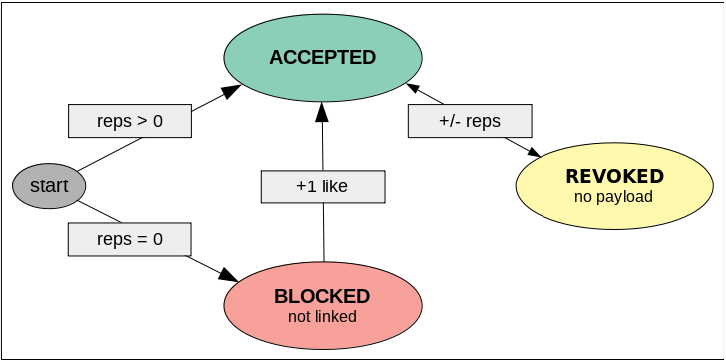
\includegraphics[width=0.65\textwidth]{state-revoked.png}
\caption{
    State machine of posts:
    \code{BLOCKED} posts are not linked in the DAG.
    \code{ACCEPTED} posts are linked and retransmitted.
    The payload of \code{REVOKED} posts are not retransmitted.
}
\label{fig.state}
\end{figure}

Finally, we consider that revoking posts is fundamental in the context of
social content publishing, and thus, an important contribution of this work.

As described in Figure~\ref{fig.state}, a forum post has three possible states:
\code{BLOCKED}, \code{ACCEPTED}, or \code{REVOKED}.
%
If the author has reputation, a new post is immediately \code{ACCEPTED} in the
forum.
%
Otherwise, it is \code{BLOCKED} and requires a like from another user.

Blocked posts are not considered part of the forum DAG in the sense that new
posts do not link back to it.
In addition, peers are not required to hold blocked posts nor retransmit them
to other peers.
However, if blocked posts are not disseminated, new users will never have the
chance to be welcomed with a like.
Therefore, a reasonable policy is to hold blocked posts in a temporary bag and
retransmit them for some visibility.

Once accepted, a post becomes part of the forum and can never be removed
again, since Merkle~DAGs are immutable by design.
%Note that blocked posts that become accepted are always succeeded by a
%\emph{like} (Figure~\ref{fig.forum}).
%
However, if the number of dislikes exceeds an arbitrary threshold (e.g., more
dislikes than likes), the post becomes \code{REVOKED} and its payload is not
retransmitted to other peers.
Note that a post hash does not depend on its associated payload, but only on
the payload hash.
Hence, it is safe to remove the payload as long as one can prove its revoked
state.
Later, if the post receives new likes, it means that the payload is still known
somewhere and peers can request it when synchronizing again, since the post
becomes \code{ACCEPTED} again.

\subsection{Peer Synchronization and Byzantine Faults}

Similarly to Bitcoin, the underlying network protocol replicates on each peer
the full state of the Merkle-DAG representing the causal relationships between
posts.
When peers synchronize, they mutually exchange missing branches such that they
reach the same DAG structure~\cite{p2p.byz}.
As they synchronize, each peer runs the consensus algorithm locally and
verifies if all received posts are consistent.

Because the protocol relies on tamper-proof DAGs, and because each peer self
verifies the posts as they synchronize, the protocol becomes tolerant to
Byzantine faults~\cite{lamport.byz}.
%
Note that no information coming from any peer is trusted a priori.
%
For instance, a malicious peer that tries to synchronize branches with erratic
data can be detected on the first inconsistent post.
This allows the correct peer to close the connection immediately and blacklist
the malicious peer from future connections.

Therefore, although Byzantine peers may still perform some sort of denial of
service attacks in the network, they cannot modify the DAG structure, nor
create arbitrary content, nor impede that two correct nodes synchronize
directly.

\section{Public Forums in Freechains}
\label{sec.freechains}

\FC~\cite{fcs.sbseg20} is an unstructured P2P topic-based publish-subscribe
protocol, in which each \emph{chain} is a replicated Merkle-DAG representing
the causal relationships between posts.
%
The protocol operation is typical of publish-subscribe systems: an author
publishes a post to a chain, which subscribed users eventually receive.
% by synchronizing DAGs.

\begin{table}
\centering
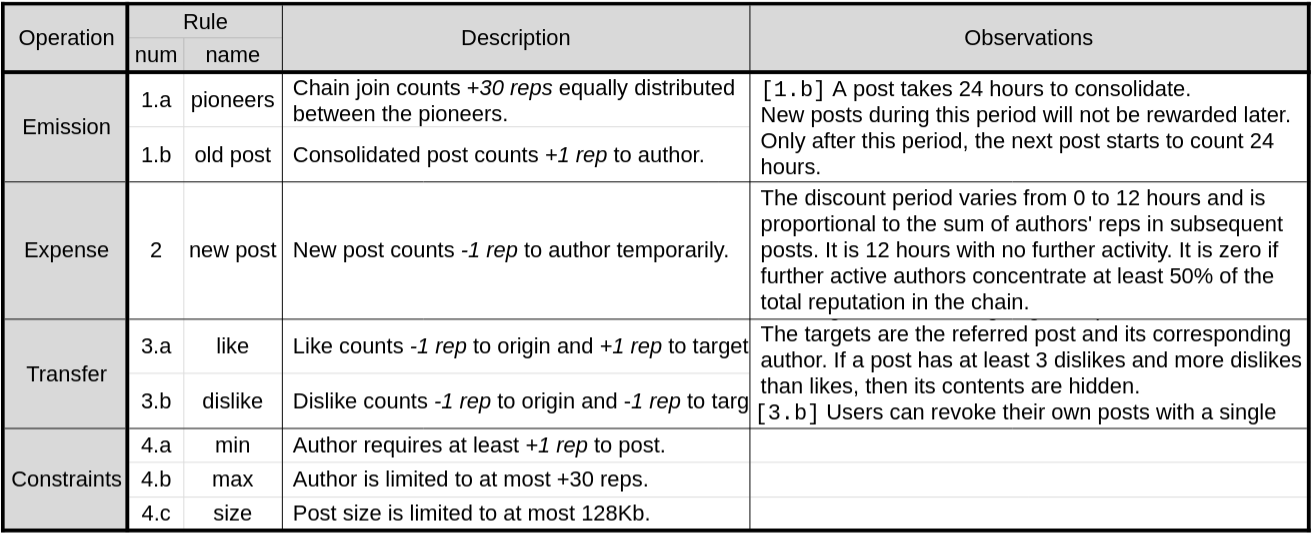
\includegraphics[width=\textwidth]{rules.png}
\caption{
    Reputation rules for public forum chains in \FC.
    The chosen constants ($30~reps$, $24h$, etc) are arbitrary and target
    typical Internet forums.
}
\label{fig.rules}
\end{table}

In order to support content moderation and mitigate abuse, we integrated the
proposed reputation and consensus mechanism of Section~\ref{sec.design} with
\FC.
Table~\ref{fig.rules} details the concrete reputation rules we conceived for
\FC, which is compatible with the general rules of Table~\ref{fig.general}, and
which are discussed as follows through an example.
Authors have to sign posts in order to be accounted by the reputation system
and operate in the chains.
We start by creating an identity whose public key is assigned as the pioneer in
a chain named \emph{forum}:

{\footnotesize
\begin{verbatim}
 > freechains keys pubpvt 'pioneer-password'
 4B56AD.. DA3B5F..  <-- public and private keys
 > freechains 'forum' join '4B56AD..'
 10AE3E..           <-- hash representing the chain
 > freechains 'forum' post --sign='DA3B5F..' 'The chain purpose is...'
 1_CC2184..         <-- hash representing the post
\end{verbatim}
}

The \code{join} command in rule~\code{1.a} bootstraps a public chain,
assigning \nreps{30} equally distributed between an arbitrary number of
pioneers indicated through their public keys (one in this example).
The pioneers shape the initial culture of the chain with the first posts and
likes, while they gradually transfer \reps to other authors, which also
transfer to other authors, expanding the community.
%
The \code{post} command in sequence is signed by the single pioneer and
indicates the purpose of the chain for future users.

%already in the community vouch for new users, or (ii) imposing explicit costs
%for new posts, such as proof of work.
%The most basic concern in public forums is to resist Sybil attacks.
%Fully P2P systems cannot rely on logins or {\footnotesize CAPTCHAs} due to the
%lack of a central authority.
%Viable alternatives include (i) building social trust graphs, in which users
%already in the community vouch for new users, or (ii) imposing explicit costs
%for new posts, such as proof of work.
%
%We propose a mix between trust graphs and economic costs.
%
In order to resist Sybils, we propose a mix between building social trust
graphs and imposing explicit costs for new posts:
Rule~\code{4.a} imposes that authors require at least \onerep to post,
effectively blocking Sybil actions.
To vouch for new users, rule~\code{3.a} allows an existing user to like a
newbie's post to unblock it, but at the cost of \onerep.
This cost prevents that malicious members unblock new users indiscriminately,
which would be a breach for Sybils.
For the same reason, rule~\code{2} imposes a temporary cost of \onerep for
each new post.
%
Note that the pioneers rule~\code{1.a} solves the chicken-and-egg problem
imposed by rule~\code{4.a}: if new authors start with no \reps, but require
\reps to operate, it is necessary that some authors have initial \reps to boot
the chains.

In the next sequence of commands, a new remote user joins the same public chain
and posts a message, which is welcomed with a like signed by the pioneer:

{\footnotesize
\begin{verbatim}
 > freechains keys pubpvt 'newbie-password'
 503AB5.. 41DDF1..  <-- public and private keys
 > freechains 'forum' join '4B56AD..'
 10AE3E..           <-- same pioneer as before
 > freechains 'forum' post 'Im a newbie...' --sign='41DDF1..'
 2_C3A40F..         <-- blocked post
 > freechains 'forum' like '2_C3A40F..' --sign='DA3B5F..'
 3_59F3E1..         <-- hash representing the like
\end{verbatim}
}

Note that chains with the same name but different pioneers would be
incompatible because the hash of genesis posts depends on the pioneers' public
keys.

Figure~\ref{fig.forum} illustrates the chain DAG up to the like operation.
The pioneer starts with \nreps{30} (rule~\code{1.a}) and posts the initial
message.
%
New posts penalize authors with \nreps{-1} during at most 12 hours
(rule~\code{2}), which depends on the activity succeeding (and including) the
new post.
The more activity from reputed authors, the less time the discount persists.
In the example, since the post is from the pioneer controlling all \reps in the
chain, the penalty falls immediately and she remains with \nreps{30}.
This mechanism limits the excess of posts in chains dynamically.
For instance, in slow technical mailing lists, it is more expensive to post
messages in sequence.
However, in chats with a lot of active users, the penalty can decrease to zero
quickly.

\begin{figure}
\centering
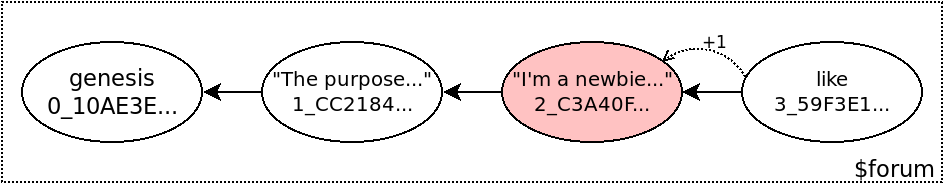
\includegraphics[width=0.65\textwidth]{forum.png}
\caption{
    The \code{like} approves the newbie message into the \code{\#forum} DAG.
}
\label{fig.forum}
\end{figure}

Back to Figure~\ref{fig.forum}, a new user with \nreps{0} tries to post a
message (hash~\code{2\_C3A40F..}) and is blocked (rule~\code{4.a}), as the red
background highlights.
But the pioneer likes the blocked message, decreasing herself to \nreps{29}
and increasing new user to \onerep (rule~\code{3.a}).
Note that the newbie post is not penalized (rule~\code{2}) because it is
followed by the pioneer like, which still controls all \reps in the chain.

With no additional rules to generate \reps, the initial \nreps{30} would
constitute the whole ``chain economy'' forever.
For this reason, rule~\code{1.b} rewards authors of new posts with \onerep,
but only after 24 hours.
This rule stimulates content creation and grows the economy of chains.
The 24-hour period gives sufficient time for other users to judge the post
before rewarding the author.
It also regulates the growth speed of the chain.
In Figure~\ref{fig.forum}, after 1 day, the pioneer would now accumulate
\nreps{30} and the new user \nreps{2}, growing the economy in \nreps{2} as
result of the two new consolidated posts.
%Note that rule~\code{1.b} rewards at most one post of each author at a time.
%Hence, extra posts during the 24-hour period do not reward authors with extra
%\reps.
%Note also that rule~\code{4.b} limits authors to at most \nreps{30}, which
%provides incentives to spend likes and thus decentralize the network, while
%rule~\code{4.c} limits the size of posts to at most \emph{128kB} to prevent
%DDoS attacks using gigantic blocked posts.

Likes and dislikes (rules \code{3.a} and \code{3.b}) serve three purposes:
    (i) welcoming new users,
    (ii) measuring the quality of posts, and
    (iii) revoking abusive posts (SPAM, fake news, etc).
%
The quality of posts is subjective and is up to users to judge them with likes,
dislikes, or simply abstaining.
%
%This way, access to chains is permissionless in the sense that the actual peers
%and identities behind posts are not directly assessed by the protocol, but
%instead by the judgement of other users in the system.
%
The reputation of a given post is the difference between its likes and
dislikes, which can be used in end-user software for filtering and highlighting
purposes.
%
On the one hand, since \reps are finite, users need to ponder to avoid
indiscriminate expenditure.
On the other hand, since \reps are limited to at most \nreps{30} per author
(rule~\code{4.b}), users also have incentives to rate content.
Hence, these upper and lower limits work together towards the quality of the
chains.
%
Note that a dislike shrinks the chain economy since it removes \reps from both
the origin and target.
Finally, the actual contents of a post may be revoked if it has at least 3
dislikes, and more dislikes than likes (rule~\code{3}).
However, considering that \reps are scarce, dislikes are encouraged to combat
abusive behavior, but not to eliminate divergences of opinion.

\subsection{Experiments with Public Forums in \FC}
\label{sec.evaluation}

We performed experiments to evaluate the performance of \FC and its consensus
algorithm.
%
As detailed further, we measure the following evaluation parameters:
    (a) metadata overhead,
    (b) consensus runtime,
    (c) graph forks, and
    (d) blocked messages.
%
The main goal of this section is to stress the consensus algorithm to show that
permissionless public forums are viable, regardless of the inherent slower
performance in comparison to permissioned protocols.

We simulate the behavior of two publicly available forums as if they were using
\FC:
%
    a chat channel from the Wikimedia Foundation%
\footnote{ Chat: \url{https://archive.org/download/WikimediaIrcLogs/} }, and
    the \emph{comp.compilers} newsgroup%
\footnote{ Newsgroup: \url{https://archive.org/download/usenet-comp} }.
%
Chats and newsgroups represent typical public forums with
    faster interactions with shorter payloads (chats), and
    slower interactions with larger payloads (newsgroups).
%
We only simulate the first \emph{10.000} messages of the forums, which
represent 3 months of activity in the chat and 9 years in the newsgroup.

The simulation spawns $N$ peers, each joining the same chain with the same
arguments.
For each message in the original forum, we
    (i)   set the timestamp of peers to match the original date,
    (ii)  create a pair of keys if the author is new,
    (iii) post the message from a random peer in $N$,
    (iv)  like the post if the author has no reputation, and
    (v)   synchronize the chain with $M$ random peers.
%
Since all messages are part of the original archive, we always perform step
(iv) to unblock messages from newbies, which we also use to measure the
evaluation parameter (d).
Step (v) will inevitably create forks in the chain for any \texttt{M<N}, which
we measure in evaluation parameter (c).

For the newsgroup, we use \texttt{N=15} and \texttt{M=5}, which represents a
larger number of peers with few interconnections to stress the local-first
nature of the protocol.
For the chat, we use \texttt{N=5} and \texttt{M=3}, which is a smaller number
of peers but with more interconnections.
%
We executed each simulation $4$ times in a desktop PC (\texttt{i7} CPU,
\texttt{8GB} RAM, \texttt{512GB} SSD).
Since the variations were negligible, we always discuss the median measures.

\begin{comment}
We assume chats are less distributed given their real-time requirements, i.e.,
users would connect to a few but more interconnected peers.
Note that \FC focus on the decentralization of authority, which is not directly
related to network distribution, which may vary from applications.
\end{comment}

Evaluation item (a) measures the protocol overhead due to blockchain metadata,
which consists of a timestamp, author signature, and hashes (post id, payload,
backlinks, and likes).
%
The original chat archive is \texttt{800kB} in size, or \texttt{80B} for each
message, which includes a timestamp, a username, and the actual payload.
The simulated chat chain is \texttt{8MB} in size, which indicates a $10x$
overhead.
% (\code{20100825 [03:37:43]})
% (\code{hello everyone})
% (\code{<Ashlee>})
The original newsgroup is \texttt{30MB} in size, or \texttt{3kB} for each
message, which includes a timestamp, a sender, a subject, and the actual
payload (typically much longer).
The simulated newsgroup chain is \texttt{42MB} in size, which indicates a
$50\%$ overhead.
% (\code{29 Aug 88 23:36:58 GMT})
% (\code{mark@ramid.com})
% (\code{Error messages and Yacc})
%
It is clear that the metatada overhead is not negligible, specially for short
chat messages, but decreases as the payload increases.

Evaluation item (b) accounts the consensus algorithm applied locally at each
chain.
We measured the time to sort posts in a local DAG both for the first time
(without any caches), and incrementally (from stable consensus caches).
%
For the chat chain, it takes \texttt{125s} and \texttt{50ms} for the initial
and incremental sorts respectively, while for the newsgroup chain, it takes
\texttt{100s} and \texttt{70ms}.
%
%Currently, we synchronize the DAGs takes hours because we the synchronization time
%
The incremental sort is limited to 7 days or 100 posts by design (as discussed
in Section~\ref{sec.design.hard}), regardless of the size of the chain, which
conveniently settles an upper bound on the input size of the consensus
algorithm.
%
Given that we use plain JSON files in the file system, we consider an
incremental consensus under \texttt{100ms} to be a practical upper bound.

Evaluation item (c) counts the number of forks in chain DAGs, which indicates
the level of asynchrony between peers following the local-first principle.
We calculate the ratio of forks over the total number of messages, e.g., a DAG
with $100$ messages and $10$ forks has a ratio of $10\%$.
%Based on the choices for $M$ and $N$ for each forum, we expect the newsgroup to
%have a higher ratio, since peers synchronize less.
We found a ratio of $18\%$ for the chat and $14\%$ for the newsgroup, which
confirms that the simulation achieves a reasonable level of asynchrony.

Evaluation item (d) measures how much bookkeeping is required to sustain active
users in the forums.
Even though the newbie rule~\code{4.a} in Table~\ref{fig.rules} is key to
combat Sybils, ideally it should not recurrently deny access to active users
with low reputation.
%
The evaluation counts the number of blocked messages requiring extra likes
after the welcoming likes (which are disconsidered) and calculates the ratio
over the total number of messages in the chain.
%This situation occurs when an user with low reputation tries to post multiple
%messages in a row without the necessary interval imposed by rule~\code{2}.
As an example, if $10$ users posted $110$ messages requiring $20$ likes, we
discount the $10$ initial messages and welcoming likes (when the user first
appears), and find a ratio of $10\%$ (\code{(20-10)/(110-10)}).
%
For the chat with $80$ users, we found a ratio of $3.7\%$.
For the newsgroup with $5000$ users, we found a ratio of $3.5\%$.
%
Considering that users were not aware of the reputation rules, the low ratios
indicate that their "natural" posting behavior matches the constraints of the
rules.
%As expected, the newsgroup has a lower bookkeeping given the higher interval
%between messages.
%
We assume that users would use the revoke mechanism to combat abusive content,
having no further effects on our evaluation.
%We also do not evaluate the quality of posts and how they would affect the
%reputation of users.

\begin{comment}
CHAT
timestamp user message
 798857 bytes

> DELL+ /x/tmp/fc-chat-20220529
- 3.7
- 455793 7419368 7875161
- erro (consensus ate 93\_*)
- 10491 / 1794 = 17%

> DELL+ /x/tmp/fc-chat-20220530
- 3.7
- 455793 7433845 7889638
- erro (consensus ate 93\_*)
- 10510 / 1851 = 18%

> DELL- /x/tmp/fc-chat-20220529
- 3.7
- 455793 7434379 7890172
- 125s, 50ms
- 10511 / 1852 = 18%

> DELL- /x/tmp/fc-chat-20220530
- 3.7
- 455793 7433590 7889383
- 150s, 50ms
- 10510 / 1850 = 18%

> NOTE 20220530
- 5.1
 455811
7577544
- 100ms / 130ms
- 10693 / 1811 = 17%

> NOTE 20220531
- 3.7
 455793
7434804
- 100ms / 130ms
- 10511 / 1851 = 18%

> NOTE 20220601
- 3.5
 455793
7384694
- 249s / 100ms
- 10456 / 1837 = 18%

-------------------------------------------------------------------------------

USENET
code From: Subject: Date: BODY
29.863.335 bytes

> DELL+ /x/tmp/fc-usenet-20220531
- 8.9
42.262.616
- 73s / 66ms
- 15659 / 2395

> DELL+ /x/tmp/fc-usenet-20220601
- 8.9
42357914
- 75s / 70ms
- 15682 / 2195

> DELL+ /x/tmp/fc-usenet-20220602
- 8.9
- 69s / 66ms
- 15669 / 2286

> DELL+ /x/tmp/fc-usenet-20220603
- 3.5
- 64s / 64ms
- 15416 / 2327

> DELL+ /x/tmp/fc-usenet-20220604
- 3.4
- 64s / 66ms
- 15419 / 2329

> DELL+ /x/tmp/fc-usenet-20220605
- 3.3
- 65s / 64ms
- 15391 / 2324

> DELL- /x/tmp/fc-usenet-20220601
- 8.7
42160398
- 52s / 70ms
- 15665 / 2198 = 14%

> DELL- /x/tmp/fc-usenet-20220602
- 60s / 70ms
- 15678 / 2091 = 13%

- lockdown strategy ok?

Discussion:
- do not scale
    - restart
- cannot evaluate behavior
    - dislike is immediate
- users are not aware of the policies
    -
- no images, videos
    - 128k enough for memes?

- Two cases
    - chat:
        - 2010-08-25 2012-11-01
        - 166277 messages
        - 13726470 bytes w/  metadata (date/time/user+msg)
        - 8592725 bytes w/o metadata (only msg)
        - 82/50 bytes/message (w/-w/o metadata)
        - 651 users
        - 227 messages per day

    - forum:
        - 1987-08-17 2012-05-28
        - 35366 messages
        - 117458214 bytes w/ metadata (date/time/user/*/+msg)
        - 3321 bytes/message
        - 13000 users
        - 3.8 messages per day

- number of forks
    - chat 30s per peer
    - e-mail 1h per peer
- time of consensus
\end{comment}

\section{Related Work}
\label{sec.related}

Many other systems have been proposed for decentralized content
sharing~\cite{p2p.survey,p2p.ecosystem}.
Here we consider the classes of publish-subscribe, federated, and P2P
protocols.

%\subsection{Publish-Subscribe Protocols}

Decentralized topic-based publish-subscribe protocols, such as
    \emph{XMPP}~\cite{pubsub.xmpp},
    \emph{ActivityPub}~\cite{pubsub.activitypub}, and
    \emph{gossipsub}~\cite{pubsub.gossipsub},
decouples publishers from subscribers in the network.
%
A key limitation of \emph{pubsubs} is that the brokers that mediate
communication still have a special role in the network, such as authenticating
and validating posts.
%
Nevertheless, some pubsubs do not rely on server roles, and instead, use
P2P gossip dissemination~\cite{pubsub.tera,pubsub.rappel,pubsub.gossipsub}.
%,pubsub.stan,pubsub.vitis
Most of these protocols focus on techniques to achieve scalability and
performance, such as throughput, load balancing, and real-time relaying.
%
However, these techniques alone are not sufficient to operate permissionless
networks with malicious Sybils~\cite{pubsub.gossipsub2}.
Being generic protocols, pubsubs are typically unaware of the applications
built on top of them.
%
In contrast, as stated in Section~\ref{sec.freechains}, the pubsub of \FC is
conceptually at the application level and is integrated with the semantics of
chains, which already verifies posts at publishing time.
For instance, to flood the network with posts, malicious peers need to spend
reputation, which takes hours to recharge (rule~\code{2} in
Table~\ref{fig.rules}).
In addition, blocked posts (Figure~\ref{fig.state}) are not a concern either,
because they have limited reachability.
Another advantage of a tighter integration between the application and protocol
is that Merkle~DAGs simplify synchronization, provide persistence, and prevent
duplication of messages.
%
In summary, \FC and \emph{pubsub} middlewares operate at different network
layers, which suggests that \FC could benefit of the latter to manage the
interconnections between peers.

%\subsection{Federated Protocols}

Federated protocols, such as e-mail, allow users from one domain to exchange
messages with users of other domains.
\emph{Diaspora}, \emph{Matrix}, and \emph{Mastodon} are recent federations for
social media, chat, and microblogging~\cite{p2p.ecosystem}, respectively.
%
As a drawback, identities in federations are not portable across domains, which
may become a problem when servers shutdown or users become unsatisfied with the
service~\cite{fed.distributed}.
In any of these cases, users have to grab their content, move to another
server, and announce a new identity to followers.
%
Moderation is also a major concern in federations~\cite{p2p.ecosystem}.
As an example, messages crossing domain boundaries may be subject to different
policies that might affect delivery.
With no coordinated consensus, it is difficult to make pervasive public forums
practical.
%
For this reason, Matrix supports a permissioned moderation system%
\footnote{Matrix moderation: \url{https://matrix.org/docs/guides/moderation}},
but which applies only within clients, after the messages have already been
flooded in the network.
%
As a counterpoint, federated protocols seem to be more appropriate for
real-time applications such as large chats rooms.
The number of hops and header overhead can be much smaller in client-server
architectures compared to P2P systems, which typically include message signing,
hash linking, and extra verification rules (as evaluated in
Section~\ref{sec.evaluation}).

%\subsection{Peer-to-Peer Protocols}

Regarding P2P protocols, Bitcoin~\cite{p2p.bitcoin} is probably the most
successful permissionless network, but serves specifically for electronic
cash.
IPFS~\cite{p2p.ipfs} and Dat~\cite{p2p.dat} are data-centric protocols for
hosting large files and applications, respectively.
Scuttlebutt~\cite{p2p.scuttlebutt} and Aether~\cite{p2p.ecosystem} are closer
to \FC goals and cover human communication.

Bitcoin adopts proof-of-work to achieve consensus, which does not solve the
centralization issue entirely, given the high costs of equipment and energy.
Proof-of-stake is a prominent alternative~\cite{p2p.proofs} that acknowledges
that centralization is inevitable, and thus uses a function of time and wealth
to elect peers to mint new blocks.
As an advantage, these proof mechanisms are generic and apply to multiple
domains, since they depend on extrinsic resources.
% (i.e., the richer gets richer)
In contrast, we chose an intrinsic resource, which is authored content in the
chains themselves.
We believe that human work grows more linearly with effort and is not directly
portable across chains with different topics.
These hypotheses support the intended decentralization of our system.
%
Another distinction is that generic public ledgers require permanent
connectivity to avoid forks, which opposes our local-first principle.
This is because a token transaction only has value as part of the longest
chain.
This is not the case for a local message exchange between friends, which has
value in itself.

IPFS~\cite{p2p.ipfs} is centered around immutable content-addressed data, while
Dat~\cite{p2p.dat} around mutable pubkey-addressed data.
IPFS is more suitable to share large and stable content such as movies, while
Dat is more suitable for dynamic content such as web apps.
%
Both IPFS and Dat use DHTs as their underlying architectures, which are optimal
to serve large and popular content, but not for search and discovery.
In both cases, users need to know in advance what they want, such as the exact
link to a movie or a particular identity in the network.
%
On the one hand, DHTs are probably not the best architecture to model
decentralized human communication with continuous feed updates.
On the other hand, replicating large files across the network in Merkle~DAGs is
also impractical.
An alternative is to use DHT links in Merkle payloads to benefit from both
architectures.

Scuttlebutt~\cite{p2p.scuttlebutt} is designed around public identities that
follow each other to form a graph of connections.
This graph is replicated in the network topology as well as in data storage.
For instance, if identity $A$ follows identity $B$, it means that the computer
of $A$ connects to $B$'s in a few hops and also that it stores all of his posts
locally.
Note however that the basic unit of communication in Scuttlebutt is
unidirectional , with a public identity broadcasting a feed to its
followers (\Xon).
%
For open groups communication (\Xnn), Scuttlebutt uses the concept of channels,
which are in fact nothing more than hash tags (e.g. \emph{\#sports}).
Authors can tag posts, which appear not only in their feeds but also in local
virtual feeds representing these channels.
However, users only see channel posts from authors they already follow.
In practice, channels simply merge friends posts and filter them by tags.
In theory, to read all posts of a channel, a user would need to follow all
users in the network (which also implies storing their feeds).
A limitation of this model is that new users struggle to integrate in channel
communities because their posts have no visibility at all.
As a counterpoint, channels are safe places that do not suffer from abuse.
%
\begin{comment}
For group \Xnn communication, \FC relies on the reputation system to prevent
abuse, since new users require at least one like for visibility in the
community.
Also, a forum chain stores its own posts only, and are not simply tags over the
entire content in the network.
\end{comment}

Aether~\cite{p2p.ecosystem} provides P2P public communities aligned with public
forums of \FC (\Xnn).
A fundamental difference is that Aether is designed for ephemeral, mutable
posts with no intention to enforce global consensus across peers.
Aether employs a very pragmatic approach to mitigate abuse in forums.
It uses established techniques, such as proof-of-work to combat SPAM, and an
innovative voting system to moderate forums, but which affects local instances
only.
In contrast, \FC relies on its permissionless reputation and consensus
mechanisms for moderation.

\section{Conclusion}
\label{sec.conclusion}

In this paper, we propose a permissionless consensus and reputation mechanism
for social content sharing in P2P networks.
We enumerate three main contributions:
    (i)   human authored content as a scarce resource
          (\emph{proof-of-authoring});
    (ii)  diversified public forums, each as an independent blockchain with
          subjective moderation rules; and
    (iii) abusive content removal preserving data integrity.

The key insight of the consensus mechanism is to use the human authoring
ability as a scarce resource to determine consensus.
This contrasts with extrinsic resources, such as CPU power, which are
dispendious and not evenly distributed among people.
%
Consensus is backed by a reputation system in which users can rate posts with
likes and dislikes, which transfer reputation between them.
The only way to forge reputation is by authoring new content under the
judgement of other users.
This way, reputation generation is expensive, while verification is cheap and
decentralized.

The reputation and consensus mechanism is integrated into \FC, a P2P protocol,
in which users can create public forums of interest and apply diverse
moderation policies.
In particular, users can revoke content considered abusive according to the
majority, not depending on centralized authorities.
%
We simulate the behavior of existing chat and newsgroup forums as if they were
using \FC to show the practicability of the protocol as a descentralized
alternative for public forums.

Finally, we do not claim that the proposed reputation system enforces ``good''
human behavior in any way.
Instead, it provides a transparent and quantitative mechanism to help users
understand the evolution of forums and act accordingly.
Human creativity contrasts with plain economic resources (e.g.,
proof-of-work), which do not appraise social interactions and also tend
to concentrate power over the time.
%
\begin{comment}

where else can we use this?
    - reddit

- Users can fork or recreate the chain.
  Unlike bitcoin, the value is not on the size, but the cohesion is users.
- Safe for niche topics and minority groups
- Fulfill the expectations of part of the community
- Part from the principle that the pioneers want it to decentralize, otherwise would create a public identity chain fig2

- INSIGHT
 Uso descentralizado
 Emissão descentralizada e restrita
 Criação difícil / Verificação fácil

- users that work twice, bots

- summary
    - parallel w/ bitcoin
        - ponte entre reputacao -> sybil -> consenso
    - no problem w/ forks
    We reach a similar solution to Bitcoin but adapted to our domain
    - we need consensus to make the reputation system work
    - we need reputation system to reach consensus
    - same virutous cycle as bitcoin
    - The more CPU work is done, the stronger becomes the proposal, the more peers
        follow it, the more tokens are mined.
        There is a strong association between work, profit and consensus that enables
        Bitcoin as a peer-to-peer cash system.
    - reputation system to rate messages
        - positively (to distinguish from excess), or
        - negatively (to block SPAM, fake news, illicit content)
    - some sort of scarcity (work)
        - you like you loose
        - you work you get
        - otherwise sybil, "likes" abuse
        - incentives for continuous, good quality posts
    - Like \emph{bitcoins}, \reps are scarce, hard to generate, and easy to verify.
      Unlike \emph{bitcoins}, \reps .

\end{comment}

\begin{comment}
- content
- CPU work to create blocks, easy objective verification, 50+1 attack, collapse
- Human work to create content, easy subjective verification, 50+1 attack,
  community fork (actually encouraged)
- unique identity based on CPU
- here based on post quality
- not CDN: Content delivery network

(b) double spend of coins/reps is solved by total ordering all
Users can like \& dislike posts, which transfer reputation between them.
Reputation is created from news

Just like Bitcoin reaches consensus with the longest chain
uses mining to

(excess, SPAM, fake, abuse, illicit)
\end{comment}

\bibliographystyle{abbrv}
\bibliography{freechains}

\end{document}
